\documentclass[%
  crop,%
  tikz,%
  multi=false%
]{standalone}%
\usepackage[utf8]{luainputenc}%
\usepackage[no-math]{fontspec}%
\defaultfontfeatures{%
  Numbers={OldStyle,Proportional},%
  Ligatures=TeX,%
  Extension=.ttf,%
}%
\setmainfont[%
  UprightFont=*-Regular,%
  ItalicFont=*-Italic,%
  BoldFont=*-Bold,%
  BoldItalicFont=*-BoldItalic,%
]{Raleway}%
\setsansfont[%
  UprightFont=*-Regular,%
  ItalicFont=*-Italic,%
  BoldFont=*-Bold,%
  BoldItalicFont=*-BoldItalic,%
]{Raleway}%
\usepackage[frenchmath]{mathastext}%
\usepackage{amsmath}%
\usepackage{amssymb}%
\usepackage{mathrsfs}%
\usepackage{mathtools}%
\usepackage{siunitx}%
\usepackage[siunitx]{circuitikz}%
\usetikzlibrary{calc,backgrounds,arrows.meta,patterns,positioning}%
\ctikzset{bipoles/length=1.2cm}%

% Colors
\usepackage{xcolor}%
\definecolor{RoseauGreen}{HTML}{cad40e}%
\definecolor{RoseauGrey}{HTML}{adb9cb}%
\definecolor{RoseauBlue}{HTML}{234e83}%

\DeclareMathOperator{\sign}{sign}%

% Sets
\let\C\relax
\newcommand{\R}{\ensuremath{\mathbb{R}}} % Real
\newcommand{\N}{\ensuremath{\mathbb{N}}} % Natural
% \newcommand{\C}{\ensuremath{\mathbb{C}}} % Complexes
\newcommand{\B}{\ensuremath{\mathscr{B}}} % Electrical buses
\newcommand{\Ch}{\ensuremath{\mathscr{C}}} % Loads
\renewcommand{\L}{\ensuremath{\mathscr{L}}} % Lines
\renewcommand{\P}{\ensuremath{\mathscr{P}}} % Phases

% Phases
\newcommand{\arm}{\ensuremath{\mathrm{a}}}%
\newcommand{\brm}{\ensuremath{\mathrm{b}}}%
\newcommand{\crm}{\ensuremath{\mathrm{c}}}%
\newcommand{\nrm}{\ensuremath{\mathrm{n}}}%
\newcommand{\grm}{\ensuremath{\mathrm{g}}}%
\newcommand{\abrm}{\ensuremath{\mathrm{ab}}}%
\newcommand{\bcrm}{\ensuremath{\mathrm{bc}}}%
\newcommand{\carm}{\ensuremath{\mathrm{ca}}}%
\newcommand{\anrm}{\ensuremath{\mathrm{an}}}%
\newcommand{\bnrm}{\ensuremath{\mathrm{bn}}}%
\newcommand{\cnrm}{\ensuremath{\mathrm{cn}}}%
\newcommand{\agrm}{\ensuremath{\mathrm{ag}}}%
\newcommand{\bgrm}{\ensuremath{\mathrm{bg}}}%
\newcommand{\cgrm}{\ensuremath{\mathrm{cg}}}%
\newcommand{\ngrm}{\ensuremath{\mathrm{ng}}}%
\newcommand{\abcrm}{\ensuremath{\mathrm{abc}}}%
\newcommand{\abcnrm}{\ensuremath{\mathrm{abcn}}}%

% Transformer
\newcommand{\Xrm}{\ensuremath{\mathrm{X}}}%
\newcommand{\Yrm}{\ensuremath{\mathrm{Y}}}%
\newcommand{\Zrm}{\ensuremath{\mathrm{Z}}}%
\newcommand{\xrm}{\ensuremath{\mathrm{x}}}%
\newcommand{\yrm}{\ensuremath{\mathrm{y}}}%
\newcommand{\zrm}{\ensuremath{\mathrm{z}}}%
\newcommand{\Arm}{\ensuremath{\mathrm{A}}}%
\newcommand{\Brm}{\ensuremath{\mathrm{B}}}%
\newcommand{\Crm}{\ensuremath{\mathrm{C}}}%
\newcommand{\Nrm}{\ensuremath{\mathrm{N}}}%

% Indices or exponents
\newcommand{\cons}{\ensuremath{\mathrm{cons.}}}%
\renewcommand{\prod}{\ensuremath{\mathrm{prod.}}}%
\newcommand{\theo}{\ensuremath{\mathrm{th.}}}%
\newcommand{\const}{\ensuremath{\mathrm{const.}}}%

% Variables
\newcommand{\umax}{\ensuremath{U^{\max}}}%
\newcommand{\umaxnorm}{\ensuremath{U^{\max\,\text{norm.}}}}%
\newcommand{\umin}{\ensuremath{U^{\min}}}%
\newcommand{\uminnorm}{\ensuremath{U^{\min\,\text{norm.}}}}%
\newcommand{\unom}{\ensuremath{U^{\text{nom.}}}}%
\newcommand{\unomnorm}{\ensuremath{U^{\text{nom.}\,\text{norm.}}}}%
\newcommand{\uup}{\ensuremath{U^{\text{up}}}}%
\newcommand{\uupnorm}{\ensuremath{U^{\text{up}\,\text{norm.}}}}%
\newcommand{\uupprime}{\ensuremath{U^{\text{up}\,\prime}}}%
\newcommand{\udown}{\ensuremath{U^{\text{down}}}}%
\newcommand{\udownnorm}{\ensuremath{U^{\text{down}\,\text{norm.}}}}%
\newcommand{\udownprime}{\ensuremath{U^{\text{down}\,\prime}}}%
\newcommand{\smax}{\ensuremath{S^{\max}}}%
\newcommand{\pmax}{\ensuremath{P^{\max}}}%
\newcommand{\sproj}{\ensuremath{\underline{S^{\text{proj.}}}}}%
%

\begin{document}
\ctikzset{european, straight voltages, cute inductors}%
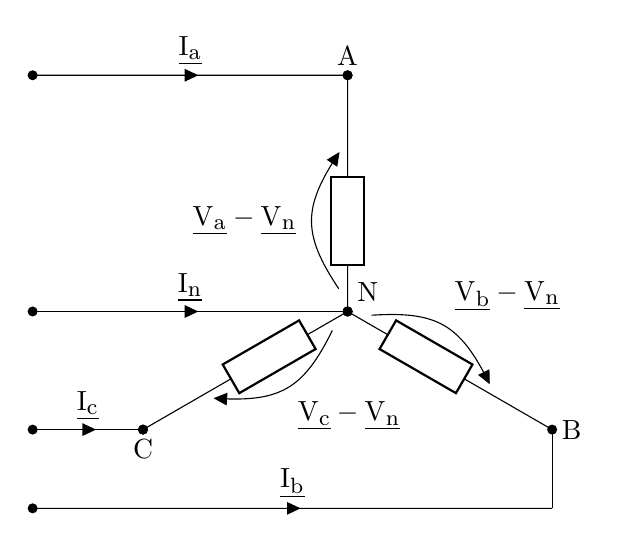
\begin{tikzpicture}[%
    show background rectangle,%
    tight background,%
    background rectangle/.style={fill=white}%
  ]
  \def\radius{2.3}%
  \def\Radius{3}%

  \ctikzset{bipoles/open/voltage/distance from node/.initial=0.1}
  % \ctikzset{bipoles/generic/voltage/european label distance=0.8}

  % Coordinates
  \coordinate (A1) at (90:\radius);%
  \coordinate (B1) at (330:\radius);%
  \coordinate (C1) at (210:\radius);%
  \coordinate (A) at (90:\Radius);%
  \coordinate (B) at (330:\Radius);%
  \coordinate (C) at (210:\Radius);%
  \coordinate (N) at (0,0);%
  \coordinate (A2) at ($(-\Radius,\Radius)-(1,0)$);%
  \coordinate (C2) at (A2 |- C);%
  \coordinate (B2) at ($(C2)-(0,1)$);%
  \coordinate (B3) at ($(B)-(0,1)$);%
  \coordinate (N2) at (A2 |- N);%

  % Nodes
  \node[above] at (A) {A};%
  \node[right] at (B) {B};%
  \node[below] at (C) {C};%
  \node[above right] at (N) {N};%

  % Lines
  \draw (A) to[short,*-] (A1) to[generic, v<=$\underline{V_{\arm}}-\underline{V_{\nrm}}$, -*] (N);%
  \draw (B) to[short,*-] (B1) to[generic, v<=$\underline{V_{\brm}}-\underline{V_{\nrm}}$, -*] (N);%
  \draw (C) to[short,*-] (C1) to[generic, v<=$\underline{V_{\crm}}-\underline{V_{\nrm}}$, -*] (N);%
  \draw (A2) to[short,i=$\underline{I_{\arm}}$,*-*] (A);%
  \draw (B2) to[short,i=$\underline{I_{\brm}}$,*-] (B3);%
  \draw (B3) -- (B);%
  \draw (C2) to[short,i=$\underline{I_{\crm}}$,*-*] (C);%
  \draw (N2) to[short, i=$\underline{I_{\nrm}}$, *-] (N);%

  % Line-to-line voltage
  % \draw (A) to[open, v=$V_{m,\abrm}$] (B)
  % to[open, v=$V_{\bcrm}$] (C)
  % to[open, v=$V_{\carm}$] (A);
\end{tikzpicture}
\end{document}
% Local Variables:
% mode: latex
% TeX-engine: luatex
% TeX-source-correlate-method-active: synctex
% ispell-local-dictionary: "british"
% coding: utf-8
% LaTeX-indent-level: 2
% fill-column: 120
% End:
